\input /Users/davidmcallester/Icloude/tex/SlidePreamble.tex
\input /Users/davidmcallester/Icloude/tex/preamble.tex

\begin{document}

{\Huge

  \centerline{\bf TTIC 31230, Fundamentals of Deep Learning}
  \bigskip
  \centerline{David McAllester, Autumn 2021}

  \vfill
  \centerline{\bf MuZero}
  \vfill
  \vfill

  \slide{Playing Blind}

{\bf Mastering Atari, Go, chess and shogi by planning with a learned model}, Schrittweiser et al., Nature 2020.

\vfill
In alpha zero we have a state (the board) and procedure for updating the state for each action.

\vfill
A representation of the board is fed to the value and policy networks.

\vfill
In mu zero no state representation is provided.  The system is only given an action set and rewards for acting.


\slide{The Algorithm}

The algorithm is very similar to alpha zero but with the addition of a state transition RNN $g_\Phi$ satisfying

\vfill
$$r^k,s^k = g_\Phi(s^{k-1},a^k)$$

\vfill
Given the state model we can perform Monte Carlo tree search (MCTS) as in alpha zero.

\vfill
Alpha zero is modified to allow intermediate reward, to use discounted reward, and to do long roll outs in addition to shallow tree searches.

\slide{The loss function}

$$\Phi^* = \argmin_\Phi \sum_k {\cal L}^\pi + {\cal L}^V +{\cal L}^R + c||\Phi||^2$$

\vfill
${\cal L}^\pi$ and ${\cal L}$ are essentially the loss functions for the policy and value respectively of alpha zero.

\vfill
The loss function function ${\cal L}^R$ trans the model RNN $g_\Phi$ to predict the rewards.  Rewards are still provided to $\mu$ Zero.

\slide{Results}

\centerline{\includegraphics[height= 4.5in]{\images/muzerochess}}

The orange line is alphazero.

\slide{Results}

\centerline{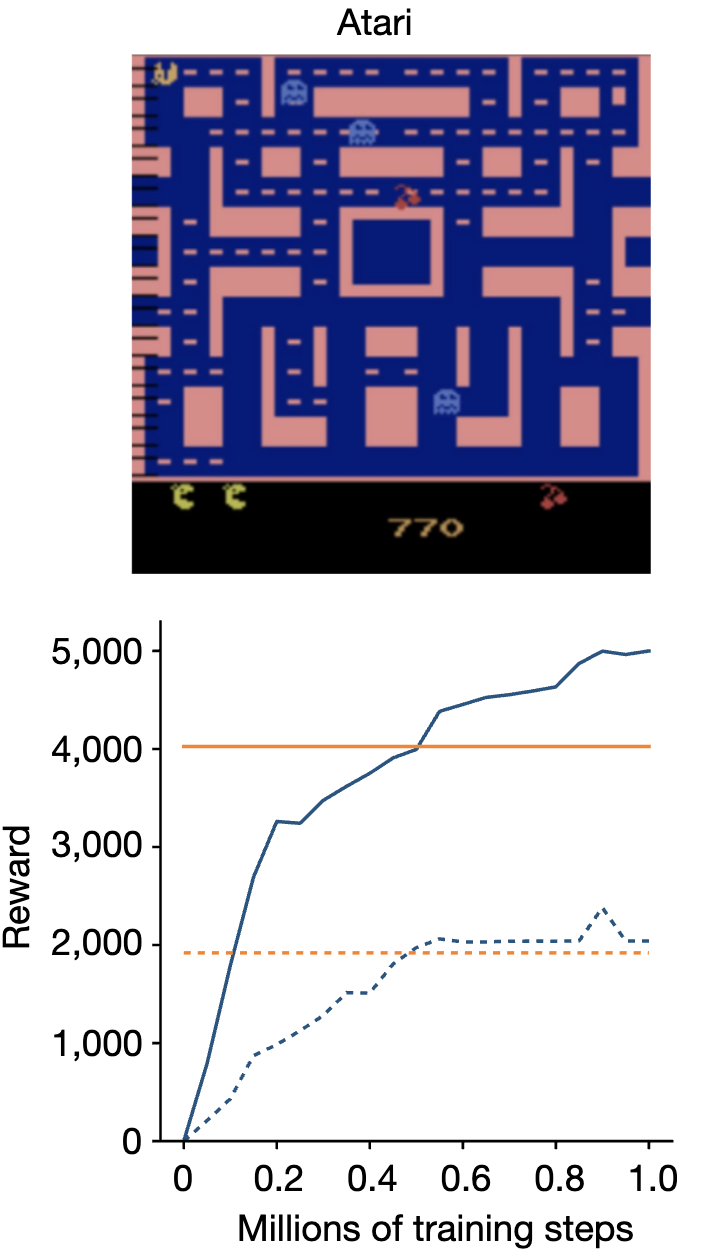
\includegraphics[height= 4.0in]{\images/muzeroatari}}

{\huge
  These are human normalized scores averaged over all 57 Atari games.  The orange line is the previous state of the art system.  Solid lines are average scores and dashed lines are median scores.
}

\slide{END}

}
\end{document}


